%%%%%%%%%%%%%%%%%%%%%%%%%%%%%%%%%%%%%%%%%
% Beamer Presentation
% Standard LaTeX Template used for creating presentation of Firebird-V Robot and other tutorials. 
% Author: Saurav Shandilya (e-Yantra Team)
% Reference: www.LaTeXTemplates.com Version 1.0 (10/11/12)
%
%%%%%%%%%%%%%%%%%%%%%%%%%%%%%%%%%%%%%%%%%

%----------------------------------------------------------------------------------------
%	PACKAGES AND THEMES
%----------------------------------------------------------------------------------------
		
\documentclass[table,10pt,red]{beamer}	% First line -- Define document class as Beamer which is used for creating presentation using Latex
\setbeamercolor{alerted text}{fg=blue} 	% Sets color of highlighted text during presentation.  
 

% The Beamer class comes with a number of default slide themes
% which change the colors and layouts of slides. Below this is a list
% of all the themes, uncomment each in turn to see what they look like.

%\usetheme{default}
%\usetheme{AnnArbor}
%\usetheme{Antibes}
%\usetheme{Bergen}
%\usetheme{Berkeley}
\usetheme{Berlin}		%used theme in present documents.
%\usetheme{Boadilla}
%\usetheme{CambridgeUS}
%\usetheme{Copenhagen}
%\usetheme{Darmstadt}
%\usetheme{Dresden}
%\usetheme{Frankfurt}
%\usetheme{Goettingen}
%\usetheme{Hannover}
%\usetheme{Ilmenau}
%\usetheme{JuanLesPins}
%\usetheme{Luebeck}
%\usetheme{Madrid}
%\usetheme{Malmoe}
%\usetheme{Marburg}
%\usetheme{Montpellier}
%\usetheme{PaloAlto}
%\usetheme{Pittsburgh}
%\usetheme{Rochester}
%\usetheme{Singapore}
%\usetheme{Szeged}
%\usetheme{Warsaw}

% As well as themes, the Beamer class has a number of color themes
% for any slide theme. Uncomment each of these in turn to see how it
% changes the colors of your current slide theme.

%\usecolortheme{albatross}
%\usecolortheme{beaver}
%\usecolortheme{beetle}
%\usecolortheme{crane}
%\usecolortheme{dolphin}
%\usecolortheme{dove}
%\usecolortheme{fly}
%\usecolortheme{lily}
%\usecolortheme{orchid}
%\usecolortheme{rose}
%\usecolortheme{seagull}
%\usecolortheme{seahorse}
%\usecolortheme{whale}
%\usecolortheme{wolverine}

%\setbeamertemplate{footline} % To remove the footer line in all slides uncomment this line
%\setbeamertemplate{footline}[page number] % To replace the footer line in all slides with a simple slide count uncomment this line

%\setbeamertemplate{navigation symbols}{} % To remove the navigation symbols from the bottom of all slides uncomment this line
%}

%------------------------------------------------------------------------------------------
%	\usepackage is required for including various features like images, table, references etc.
%	Packages must be installed before using. These can be istalled through package manager. 
%   Various packages have dependencies and for using such packages all dependent packages must be used. 
%-----------------------------------------------------------------------------------------
\usepackage{beamerthemeshadow} % theme shadow for visual 
\usepackage{beamerthemesplit} % Creates minipage (for showing multiple images and text) on same page  
\usepackage{graphicx} % Allows including images
\usepackage{booktabs} % Allows the use of \toprule, \midrule and \bottomrule in tables
\usepackage{xcolor}
\usepackage{booktabs,array}
\usepackage{listings}
\usepackage{hyperref}	% Required for including hyperlink in document
\usepackage{verbatim,moreverb} % Required for including code snippet.
\usepackage{colortbl}
\usepackage{multirow}	% Required for creating multiple row tables
\usepackage{tikz}		% Required for drawing shapes such as circles, arrowed line, etc. 
\usetikzlibrary{arrows}
\usepackage{ragged2e}

% logo
\logo{
\includegraphics[height=1cm]{iitblogo.pdf}} % includes logo at bottom of all slides 

%----------------------------------------------------------------------------------------
%	TITLE PAGE
%----------------------------------------------------------------------------------------
% sf family, bold font
\sffamily \bfseries
% content inside [] appears at bottom of all page. content inside {} appears on first page as title. double backslash means line change 
\title
[
	e-Yantra	% bottom of all page
	\hspace{0.5cm}
	\insertframenumber/\inserttotalframenumber
]
{
	Interfacing a PIR Sensor with FireBird V Robot
}

\author
[
	www.e-yantra.org 	%Name at bottom of all page 
]
% author name on title slide
{
	Shantanu Sengupta \\
\vspace{5mm}
  Embedded Real-Time Systems Lab\\
  Indian Institute of Technology-Bombay \\
}
\date
{
IIT Bombay \\ {\today}	%\today picks system date on title slide
}

\begin{document} % IN LATEX ALL DOCUMENT/REPORT/PRESENTATION STARTS WITH \begin{document} AND ENDS WITH \end{document}

\begin{frame}	% FRAME MEANS SLIDE. \begin{frame} STARTS THE SLIDE AND \end{frame} ENDS THE SLIDE
	\titlepage % Print the title page as the first slide
\end{frame}

% START OF SECOND SLIDE
\begin{frame}
	\frametitle{Agenda for Discussion} % Table of contents slide, comment this block out to remove it
	\tableofcontents % Throughout your presentation, if you choose to use \section{} and \subsection{} commands, these will automatically be printed on this slide as an overview of your presentation
\end{frame}

%----------------------------------------------------------------------------------------
%	PRESENTATION SLIDES
%----------------------------------------------------------------------------------------

%------------------------------------------------
\section{Introduction} % Sections can be created in order to organize your presentation into discrete blocks, all sections and subsections are automatically printed in the table of contents as an overview of the talk
%------------------------------------------------


% Start of Third slide
\begin{frame}
	\frametitle{Introduction}
\pause
 		
 		\color{black} 


\begin{minipage}[c]{0.6\textwidth}
			\begin{itemize}
\justifying
\item <+-|alert@+>    Passive Infrared Sensor measures Infrared light coming from objects in its field of view
\item <+-|alert@+> Everything emits some low level radiation and hotter something is, the more radiation is emitted.	
\item <+-|alert@+> The pyroelectric sensor in the PIR is split into two slots. When a body moves in its field of view, one slot experiences more IR than the other, and a differential voltage is created, which indicates the motion of a human.


\end{itemize}
		\end{minipage}
\begin{minipage}[c]{0.37\textwidth}
\hspace*{5mm}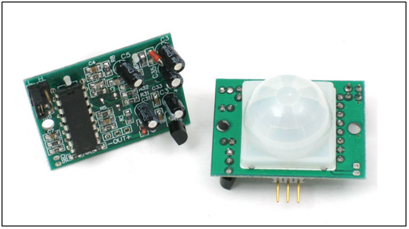
\includegraphics[width=\linewidth]{PIR_Sensor.png}
		\end{minipage}
\end{frame}

%------------------------------------------------
\subsection{Specifications}
\begin{frame}
	\frametitle{Specifications}
\pause 		
 		\color{black} 


			\begin{itemize}
\item <+-|alert@+>   Single bit output
\item <+-|alert@+> Small size makes it easy to conceal
\item <+-|alert@+> Sensitivity: Pre-settable
\item <+-|alert@+> Size: Length 32mm, Width 24mm, Thickness 26mm
\end{itemize}
		
\end{frame}





%------------------------------------------------

\section{Working Principle} 
\subsection{Principle}
 \begin{frame}
	\frametitle{Working Principle}
\pause
		\begin{itemize}
\justifying
\item <+-|alert@+>  PIR Sensor has two slots in it
\item <+-|alert@+> When idle, both slots detect the same amount of IR 
\item <+-|alert@+> When a warm body like a human or animal passes by, it first intercepts one half of the PIR sensor, which causes a positive differential change between the two halves of the PIR Sensor.
\item <+-|alert@+> When the warm body leaves the sensing area, the reverse happens, whereby the sensor generates a negative differential change.
\item <+-|alert@+> These change pulses are what is detected
\end{itemize}
		

\end{frame}

\subsection{Illustration of Working Principle}
 \begin{frame}
	\frametitle{Illustration of Working Principle}
\pause
\begin{minipage}[c]{0.80\textwidth}
\begin{center}

\hspace*{10mm}\includegraphics[width=\linewidth]{Working.png}		
\end{center}	
	\end{minipage}

\end{frame}
%-------------------------------------------------------

%------------------------------------------------

\section{Connection Details} % Sections can be created in order to organize your presentation into discrete blocks, all sections and subsections are automatically printed in the table of contents as an overview of the talk
%------------------------------------------------

\subsection{Connections of a PIR Sensor} % Sections can be created in order to organize your presentation into discrete blocks, all sections and subsections are automatically printed in the table of contents as an overview of the talk
%------------------------------------------------


% Start of Third slide
\begin{frame}
\frametitle{Connections of a PIR Sensor}
\pause
	\begin{minipage}[c]{0.52\textwidth}
\begin{itemize}
\justifying
\item <+-|alert@+>  \textbf{+V :} This pin of the PIR sensor should be connected to an
external 5V supply.
\item <+-|alert@+> \textbf{GND :} This pin of the PIR sensor should be connected to
Ground.
\item <+-|alert@+> \textbf{OUT :} This pin of the PIR sensor is the digital output. This pin
is to be read by the microcontroller to detect the movement and
decide the appropriate action that should be taken
\end{itemize}
		\end{minipage}
\begin{minipage}[h]{0.45\textwidth}
\hspace*{5mm}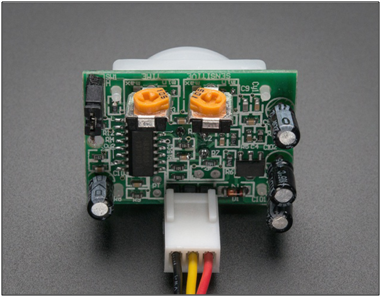
\includegraphics[width=\linewidth]{PIR_Sensor_pins.png}	
		\end{minipage}
\end{frame}



% Start of Eighth slide
\subsection{Pin Connections between PIR Sensor and FireBird V Robot} % A subsection can be created just before a set of slides with a common theme to further break down your presentation into chunks
\begin{frame}
\frametitle{Pin Connections between PIR Sensor and FireBird V Robot}
\pause
\begin{table}
\begin{tabular}{l l l}
\toprule
\textbf{Pins of PIR Sensor} & \textbf{PinsofATmega2560Microcontroller} \\
\textbf{} & \textbf{BoardExpansionSocket} \\
\midrule
GND & Pin 23/24 (or any Ground pin)\\
+V & Pin 21/22 (or any 5 Volts pin) \\
Digital Output & Any GPIO Port Pin\\
\bottomrule
\end{tabular}
\caption{Pin Connections between PIR Sensor and FireBird V Robot}
\end{table}
\end{frame}
%------------------------------------------------

\subsection{Jumper Settings}
% Start of Third slide
\begin{frame}
	\frametitle{Jumper Settings}
\pause 		
 		\color{black} 


\begin{minipage}[c]{0.6\textwidth}
There are two triggering modes available in the PIR Sensor. These modes can be changed according to the jumper positions.
			\begin{itemize}
\justifying
\pause
\item <+-|alert@+> \textbf{ H Retrigger Mode:} Output remains HIGH when sensor is retriggered repeatedly. Output is LOW when idle ie not triggered
\item <+-|alert@+> \textbf{Normal Mode: }Output goes HIGH then LOW when triggered. Continuous motion results in repeated HIGH/ LOW
pulses. Output is LOW when idle

\end{itemize}
		\end{minipage}
\begin{minipage}[c]{0.37\textwidth}

\hspace*{5mm}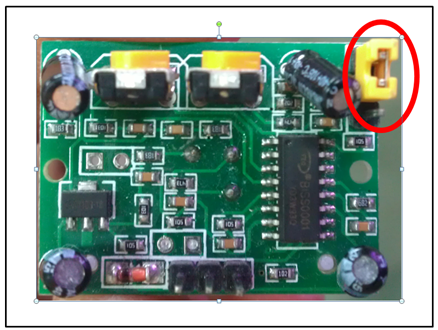
\includegraphics[width=\linewidth]{H.png}\\
\pause
\hspace*{5mm}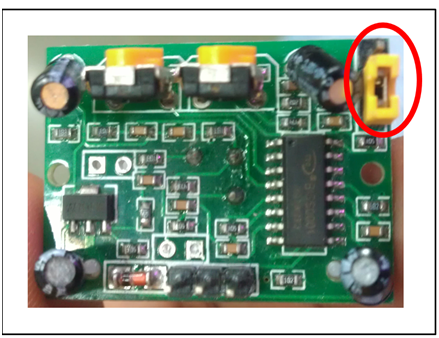
\includegraphics[width=\linewidth]{L.png}
		\end{minipage}
\end{frame}


\section{C Code} 

\begin{frame}
	\begin{center}
\huge C Code
\end{center}
\end{frame}

%------------------------------------------------

\section{Output displayed on LCD \& LED Bargraph} % Sections can be created in order to organize your presentation into discrete blocks, all sections and subsections are automatically printed in the table of contents as an overview of the talk
%------------------------------------------------

\begin{frame}
	\frametitle{Output displayed on LCD \& LED Bargraph}
\pause
\hspace{0mm}
	\begin{minipage}[c]{0.49\textwidth}
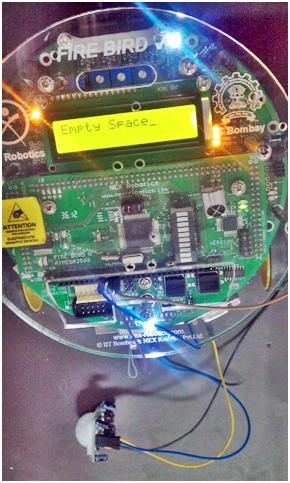
\includegraphics[width=0.8\linewidth]{out1.png}
	\end{minipage}
	\begin{minipage}[c]{0.49\textwidth}
			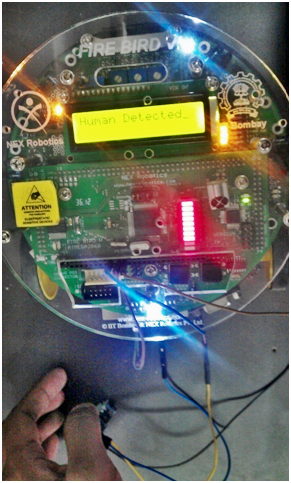
\includegraphics[width=0.8\linewidth]{out2.png}
	\end{minipage}


		
\end{frame}

\section{Applications using PIR Sensor}
% Start of Third slide
\begin{frame}
	\frametitle{Applications using PIR Sensor}
\pause
	\begin{minipage}[c]{0.45\textwidth}
\begin{itemize}
\item <+-|alert@+> Human Detection Applications
\item <+-|alert@+> Thermal Imaging
\item <+-|alert@+> Infrared Homing

\end{itemize}
		\end{minipage}
\begin{minipage}[c]{0.52\textwidth}

			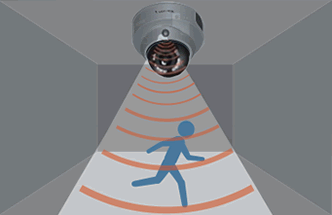
\includegraphics[width=\linewidth]{pirapp.png}\\
\pause
	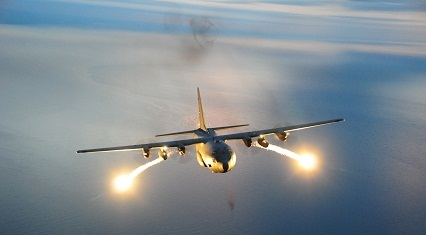
\includegraphics[width=\linewidth]{6727973.jpg}

		\end{minipage}


		
\end{frame}

\begin{frame}
	\frametitle{Thank You!!}
\pause
		\begin{center}
\large Thank You!!
\end{center}
\end{frame}
\end{document} 